\chapter{Feladat megvalósítása}
\label{ch:imp}
Mint már fentebb említésre került, a dolgozat témája részben egy valós, határidős projekt volt, így ennek megfelelően egy csapat dolgozott rajta. Ezen belül én is részfeladatokat kaptam és implementáltam, valamint részt vettem a tervezési procedúrában. 

\section{Wrapper fejlesztése QRadar-hoz}
A projekt első kihívása egy Java alapú wrapper fejlesztése volt a QRadar reference data manipulációt kezelő webes REST API-jához. Későbbiekben ezen a wrapperen keresztül bonyolítunk majd minden forgalmat az átláthatóbb kód készítése céljából, ezért fontos hogy a wrapper megvalósítson minden olyan funkciót amire szükség lehet.

A fejlesztés első lépéseként tanulmányoztam a REST API-hoz tartozó referencia dokumentációt, ami leírja mely endpointokon milyen HTTP kérések hajthatók végre, milyen paraméterekkel, milyen választ adhat és milyen státusz üzeneteket kaphatunk. Ebből az anyagból kiderült, hogy a négy reference data típushoz 4 endpoint halmaz tartozik, amelyek hasonló felépítéssel és paraméterezéssel bírnak. Egy ilyen endpoint halmazra mutat példát az alábbi felsorolás.

\begin{itemize}
	\item /sets - GET, és POST műveletet támogat. A POST-tal új reference set hozható létre, a GET metódussal pedig lekérhető a rendelkezésre álló setek listája.
		\subitem /\{name\} - GET, POST, DELETE. Az URL-ben megadott paramétert a QRadar a reference set neveként értelmezi, és ezen keresztül érhető el a set lekérése (GET), teljes törlése (DELETE), valamint egy elemi adat feltöltése (POST).
			\subsubitem /\{value\} - DELETE. Ennek az endpointnak a segítségével tudunk egy bizonyos értéket törölni a reference set-ből.
		\subitem /bulk\_load/\{name\} - POST. Az egyik legfontosabb endpoint, mivel ezen keresztül tudunk feltölteni egy olyan JSON formátumú szöveget, amellyel egyszerre több értéket is tudunk állítani egy reference setben (vagy más endpointok esetén más reference data-kban).
\end{itemize}

A fent felsorolt endpointok közül mindegyiket implementáltam a wrapperben, Java konvención alapuló neveket adva a függvényeknek. Egy függvény egy működést valósít meg, és ez a működés a reference data típusának szempontjából transzparens, tehát nem szükséges külön metódust hívni egy reference set és egy reference map feltöltéséhez, hanem elég egy metódust, más paraméterekkel.

A reference data-kkal való könnyebb interakció miatt definiáltunk egy saját adatszerkezetet egy Java osztály formájában, a data típusokkal megegyező néven. Mindegyik osztály egy ReferenceData navű absztrakt ősosztályból származik, ami egy egységes interface-t biztosít a leíró adatok, mint például a típus, az adatok típusa, lekéréséhez. Ennek a ReferenceData-nak a leszármazottai a konkrét reference típusokat megvalósító osztályok. Mindegyik osztály rendelkezik egy, a saját maga által reprezentált struktúrának megfelelő tárolóval, amely tárolja az adott reference data adatait. Mivel az integráció során többnyire szöveges, vagy azzá könnyen átalakítható adatokkal dolgozunk, és a QRadar irányába is JSON formátumban továbbítjuk az adatokat, így kézenfekvő mindet szövegként tárolni. A tárolókhoz használt kollekciók pontos típusa, valamint az implementációhoz használt architektúra leolvasható a mellékelt ábráról \ref{fig:referencedata}. 

Lehetséges lenne más formátumban tárolni az adatokat, mint például egy Java alapú JSON reprezentációban, JSONObject-ben, vagy akár egy hosszú karakterláncként is, ám ezzel elvesztenénk a Java beépített kollekciói által nyújtott funkciókat, mint például az iterációt, vagy a tartalmazás ellenőrzését. Ezek mind nélkülözhetetlen funkciók a könnyű fejlesztés érdekében, valamint a megfelelő teljesítmény biztosítása szempontjából is fontosak, amire később látunk majd példát. 

\begin{figure}
	\centering
	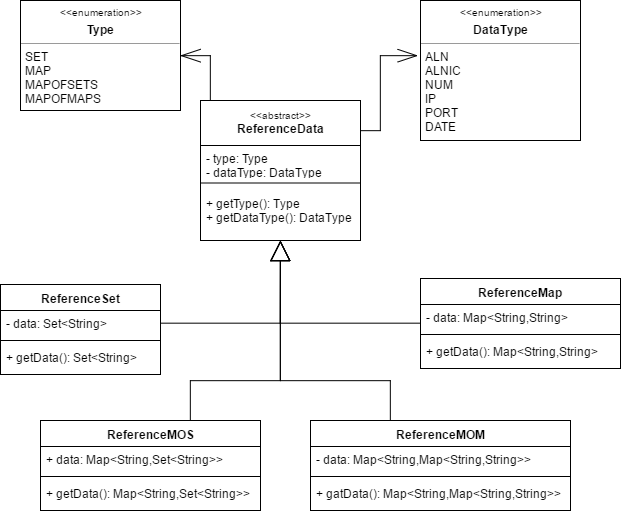
\includegraphics[width=0.7\linewidth]{figures/ReferenceData}
	\caption{A ReferenceData osztály és leszármazottainak felépítése}
	\label{fig:referencedata}
\end{figure}

A wrapper fejlesztése közben külön kihívást jelentett a QRadar REST API-val való kommunikáció megvalósítása. A QRadar ugyanis csak HTTPS forgalmat fogad el, TLS segítségével, ezért egy, a QRadar által generált tanúsítványt kellett hozzáadni minden olyan környezethez, amely a wrappert használta. Ez a két külön architektúra esetén a WebSphere és a TDI tanúsítvány könyvtárát jelentette, és ez egy olyan követelmény, ami a wrapper későbbi használata esetén is szükséges. Emellett a QRadar megköveteli, hogy a REST API-jához csatlakozó kliensek használjanak egy, a QRadar által előre generált token-t, amit minden híváskor fel kell küldeniük. A wrapper osztály ezt konstruktorában kéri, és automatikusan minden kérésnél elküldi. A TLS kapcsolat biztosítja a szerver hitelességét, míg a token a szerver számára hitelesíti az API-t használó klienst, így összességében a kommunikáció kölcsönösen hitelesített.

Magának a HTTP forgalomnak és a REST hívásoknak a lebonyolítására az Apache Wink\cite{wink} frameworköt használtam. Ez egy egyszerű Java alapú framework, melynek része egy JAX-RS kompatibilis szerver, és egy kifejezetten REST hívások lebonyolítására kiélezett HTTP kliens. A projektben a kliens komponens RestClient osztályát használtam, valamint a frameworkkel együtt érkező JSON4J csomagot, a JSON inputok parse-olására és a szöveges outputok generálására. A fejlesztés közben külön kihívást jelentett a JSON4J csomag megfelelő osztályainak használata, valamint egymásba ágyazása. Ez a csomag ugyanis két osztályt bocsájt rendelkezésre a JSONObject valamint a JSONArray formájában. Az object osztály reprezentálja a map típusú, míg az array a tömb típusú struktúrákat. Ez annyiban nehezítette a fejlesztést, hogy a különböző ReferenceData leszármazottak közt nem lehetett egységes parse-olást használni, hanem a többszörösen egymásba ágyazott kollekciók esetén több lépcsős iterációt kellett használni a JSON felépítéséhez. Ez túl nagy adathalmazoknál lassabb működést eredményezhet.

A wrapper a különböző reference data-k transzparens kezelésén túl egyéb funkciókat is ellát, mint például segéd funkciók biztosítása, vagy a hibák egységes kezelése. Ilyen segéd funkciók a különböző adattranszformációk a használt típusok és a JSON formátum között, vagy például különböző ellenőrzések egy reference data létezésére, vagy egy aszinkron törlés lefutására. A hibakezelés menedzselésére a wrapper egy saját kivétel osztályt definiál, ami minden, a sikeres lefutástól eltérő esetben (akár belső hiba, akár a QRadarral való kommunikáció közben fellépő hiba) eldobásra kerül. Ez az objektum tartalmaz egy szöveges üzenetet, ami a hiba okára utal, valamint egy státusz kódot, ami ha HTTP kommunikáció közbeni hiba történt, annak a kódját tartalmazza, ha belső működésbeli hiba (például parse-olási hiba) akkor egy 0-nál kisebb számot tartalmaz. Ez egységesen és könnyen használhatóvá teszi a felsőbb rétegek számára, ahol például logolást kezeljük, mert egyértelmű, hogy a hiba milyen forrásból adódott. A saját kivétel típus pedig tovább könnyíti a hibák elválasztását, főleg ha a wrappert egy nagyobb frameworkben használjuk.

A wrapper támogatja a QRadar által használt összes adattípust (ALN, ALNIC, IP, NUM, PORT, DATE), a REST hívások be- és kimenetét az adott típus által megkövetett JSON formátumban állítja elő/dolgozza fel.

%Ezen kívül a QRadar reference data-i támogatják még az inputok különböző típusú validációját, valamint egy elévülési információ hozzárendelését. A típus validáció abban valósul meg, hogy beállítható a reference data-ban található adat típusa, és feltöltéskor a QRadar ezt validálja, valamint feldolgozza. A típusokra az alábbi lehetőségek állnak rendelkezésre: Alphanumeric, Alphanumeric ignore case, Numeric, IP, Port, Date. 

Ezen kívül a wrapper kezeli az elévülési (TTL) paramétereket is, amelyek két részből tevődnek össze: az egyik az elévülés ideje, a másik típusa, vagyis milyen szabály alapján évüljenek el az adatok. Ennek a lehetséges értékei az UNKNOWN, a LAST\_SEEN, és a FIRST\_SEEN, amik azt határozzák meg, hogy az elévülési időt honnan számoljuk: az adott adat először bekerülésének idejétől, vagy az utolsótól. Az elévülési időt szöveges formátumban (pl.: 36 hours) várja a QRadar API-ja, amit feldolgoz, és valós idő értékekké alakít.

%Mindkét plusz funkció használatát támogatja a wrapper.

\section{TDI Integráció megvalósítása}

A TDI alapú megoldás célja egy olyan keret, és hozzá tartozó use case-ek kidolgozása, amely lehetőséget ad az ISIM és QRadar közti integrációs feladatok gyors, hatékony és egyszerű megvalósítására. 
A TDI már létező LDAP és adatbázis (JDBC) connectorral rendelkezik, ezért az ISIM adatforrásként való használata gyári komponensekkel oldható meg. A QRadar API használatához viszont új connector fejlesztésére volt szükség.
Mivel a TDI által nyújtott keretrendszerbe illeszkedik a megoldás, így képes használni az általa nyújtott számos lehetőséget, például a már létező connectorokat sokféle rendszerhez, valamint a use case implementációk alapján később könnyedén készíthetők új megoldások olyanok által, akik járatosak a TDI használatában. 

A megvalósításhoz szükség volt elsősorban egy connector létrehozására, majd ezt felhasználva implementáltam több lekérdezés típust, általunk, valamint az ügyfél által definiált esetekre.

 
\subsection{QRadar connector fejlesztése TDI-hoz}\label{subsec:connimpl}

A TDI alapú megoldás első lépése egy connector fejlesztése volt a TDI és a QRadar közti integrációhoz. Ehhez segítségemre volt a hivatalos útmutató connector fejlesztéshez. \cite{conndev} 

Egy saját connector fejlesztése TDI alatt abból áll, hogy létrehozunk egy új Java osztályt ami implementálja a megfelelő, TDI által specifikált interfészt, ennek metódusain belül elkészítjük a kívánt üzleti logikát. Majd készítünk egy xml alapú leíró fájlt, ami meghatározza a TDI számára, hogy a connector milyen paramétereket vár, azokat milyen formában, valamint a felhasználói felületen az egyes paraméterekhez milyen GUI elemek tartozzanak. Ezt a leírót, valamint a lefordított .class fájlokat a megfelelő struktúrában becsomagoljuk egy JAR fájlba, amit a TDI által használt könyvtárak egyikébe másolunk. 

Egy connector-nak nyolc működési módja lehet, amit a feljebb említett dokumentum pontosabban is specifikál. Ezek a következők:


\begin{itemize}
	\item Iterator - Végigiterál az adatforrás elemein, azokat felolvassa, és az assembly line rendelkezésére bocsájtja.
	
	\item AddOnly - Az assembly line-on érkező adatokat hozzáadja az adatforráshoz.
	
	\item Lookup - Egy kritérium alapján keresést hajt végre az adatforráson és kiválasztja a kritériumra illeszkedő elemet vagy elemeket. Jellemzően több adatforrás elemeinek illesztésére használatos.
	
	\item Delete - Az assembly line-ról kapott összes elem esetén a megadott kritériumot felhasználva megkeresi az elemet, és ha megtalálta, törli azt. Lehetőség van olyan felparaméterezésre is, amely egyszerre több elemet töröl.
	
	\item Update - Már meglévő adatok módosítását végzi. Előbb  megkeresi a megadott kritérium alapján a rekordokat, ha talált ilyen elemet, akkor összehasonlítja az assembly line-on érkező elemmel, és elvégzi a szükséges módosításokat. Ha nem talált megfelelő elemet, akkor hozzáadja újként.
	
	\item Delta - Egy különleges mód, melyhez szükség van további, ilyen módot támogató elemekre az assembly line-on. A felolvasott adatokat összehasonlítja egy külső tárolóban (ún. delta store) tárolt elemekkel, és a két elem differenciáiból delta műveleteket képez, amiket végrehajt a célrendszeren. Eltárolja a kezelt elemek legutóbb használt verzióját, és csak az újonnan beolvasott elemekhez képesti különbséget hajtja végre.
	
	\item Server - Ebben a módban a connector egy szerver típusú viselkedést valósít meg, ahol vár egy bejövő kapcsolatra (TCP, LDAP, HTTP, stb.), aminek a hatására egy új szálon elindítja a saját assembly line-ja egy másolatát, ami a beérkező adatokkal végrehajtja a feladatot, választ küld a bejövő kérésre, majd terminálódik. Az eredeti példány közben újabb kapcsolatokra vár.
	
	\item CallReply - Egy speciális mód, ami olyan interakciók végrehajtására lett tervezve, amelyeknél attribútumok transzformációját (vagy új attribútum előállítását) a connector által kezelt külső komponens végzi. Működése a lookup módhoz hasonló, azzal a különbséggel, hogy keresési kritérium helyett egy attribútumhalmazt halmazt adunk át, amelyen tetszőleges műveletet végrehajthat a külső komponens. A connector ilyenkor be- és kimenetei attribútumokkal is rendelkezik.
\end{itemize}

Egy connector nem feltétlenül támogat minden módot, a támogatni kívánt módok határozzák meg, hogy a fejlesztendő connectornak milyen metódusokat kell implementálnia a megfelelő működéshez. 
Például az AddOnly mód csak az Initialize, putEntry, és a terminate metódusokat használja, így ha a connector csak ezt akarja használni, elég ezeket implementálni. Ezzel szemben például az Update mód ezeken felül használja a findEntry, és a modEntry metódust is. Minden connector a saját logikáját definiálja, amivel megvalósítja az adott célrendszeren az absztrakt módon megfogalmazott műveletet. Egy JDBC connector például adatbázis parancsokkal valósítja meg a fent definiált műveleteket egy kapcsolaton keresztül. Jelen esetben egy REST API-n keresztül elérhető a kommunikáció a célrendszerrel, így a connector szabványos HTTP kéréseket használ. A fejlesztés során megvalósításra került az összes fent említett mód, kivéve a Server, és a CallReply, mivel ezek a konkrét kontextusban nem értelmezhetőek.

Első lépésként tehát elkészítettem egy QRadarReferenceDataConnector osztályt, ami örököl egy generikus ősosztályból, ami már előre megvalósít olyan metódusokat a TDI által használt ConnectorInterface-en, amelyek nem kifejezetten connector specifikusak, hanem generikus feladatokat látnak el, például konfigurációs fájlok beolvasása vagy paraméterek beállítása.

Az implementációs döntések megértéséhez fontos ismerni egy connector életciklusát. A connector létrejöttekor meghívódik a konstruktora, de ez a dokumentációban leírtaknak megfelelően nem szabad, hogy paraméter és egyéb beállításokat tartalmazzon, mert a példány már létrejöhet az előtt, hogy a szükséges paraméterek beolvasásra kerültek. Ez azért történhet meg, mert ezt a konstruktort használja a TDI grafikus felülete a kezdeti beállítási és paraméterezési felület elkészítéséhez. A konfiguráló, valamint az erőforrás foglaló műveletek ezért az Initialize metódusban kaptak helyet, ami az assembly line futás elején hívódik meg. A connector objektum egészen az assembly line végéig életben marad, majd az assembly line lezárultakor lefut a terminate metódusa. Erre azért van szükség, hogy a connector megfelelően felszabadíthassa az általa foglalt erőforrásokat és a nyitott kapcsolatokat.

A connector életciklus ismeretében, valamint a QRadar és a REST API-jának működése és teljesítményének optimalizálása miatt úgy döntöttünk, hogy az assembly line futása közben nem azonnal kerülnek fel az adatok a QRadar megfelelő reference data-jába, hanem azok először a connector egy változójában akkumulálódnak, és az életciklus végén, a terminate metódus hívásakor kommittálódnak. Két ilyen változót használtam, egyet a törlendő, egyet az újonnan hozzáadandó elemek tárolására. A megvalósítás valamint a wrapper használata miatt adott volt, hogy ezeknek az akkumulátor változóknak a megvalósítását a QRadarApiWrapper mellé fejlesztett ReferenceData osztály, valamint leszármazottjai szolgáltassák.

Az alábbi metódusokat implementáltam a connector által támogatott metódusokhoz:

\begin{itemize}
	\item initialize - Az inicializálást végrehajtó metódus. Alapértelmezetten az assembly line indulásakor hívódik meg. Lekéri az ősosztály segítségével a felületen megadott paramétereket és azokat megfelelő formátumra hozza, valamint inicializálja az olyan attribútumokat, amelyek a paraméterezés alapján más értékeket vehetnek fel. Emellett ha az opció használatban van, akkor létrehozza az új reference data-t.
	
	\item findEntry - Keresést végrehajtó metódus. A megadott SearchCriteria alapján végrehajt egy keresést a kiválasztott reference data elemein. Mivel a QRadar API nem definiál keresés műveletet, a keresést egy előzetesen letöltött teljes adathalmazon kell végrehajtani. Elkerülendő, hogy minden egyes findEntry híváskor újra le kelljen kérdezni a teljes adathalmazt, ez a metódus egy gyorsítótárazási megoldást használ. Az első keresésnél lekérdezi a teljes reference data-t, majd ebben a lokális példányban keres az összes többi futása során. 
	
	\item  putEntry - Hozzáadást, azaz adat kiírást végrehajtó metódus. A paraméterként kapott entry-t feldolgozza, és a connector számára értelmezett kulcsok (\textit{value},\textit{key},\textit{inner\_key}, \textit{payload}) mentén hozzáadja őket a megfelelő akkumulátorokhoz. Ha payload érkezik, amit egy az egyben továbbítunk a QRadar felé, akkor egy String-eket tartalmazó listához adja hozzá, ha key, value, inner\_key formátumban érkezik adat, akkor pedig a megfelelő reference data akkumulátorhoz.
	
	\item modEntry - Módosítást végrehajtó metódus. Először feldolgozza a paraméterként kapott új entry-t, a régi entry-t, valamint a keresési feltételeket az alapján, hogy milyen típusú reference data-t kell módosítania. Ezután mind a négy típusra végrehajtja a szükséges lépéseket a sikeres módosításhoz. Ezek a következők:
	\begin{itemize}
		\item Set: A régi értéket hozzáadja a törlendőket tartalmazó akkumulátorhoz, az újat pedig a hozzáadandóakhoz
		
		\item Map: Ha az új érték kulcsa nem egyezik a régi érték kulcsával, akkor a régi értéket hozzáadja a törlendőket tartalmazó akkumulátorhoz, az újat pedig a a hozzáadandóakhoz.
		
		\item Map of sets: A sethez hasonlóan, a régi értéket a törlendőhöz, az újat a hozzáadandóhoz adja.
		
		\item Map of maps: A maphez hasonlóan ellenőrzi, hogy a key, valamint az inner\_key megegyezik e, ha nem, akkor hozzáadja a törlendőhöz a régit, az újat pedig a hozzáadandóhoz.
	\end{itemize}

	\item deleteEntry - Törlésért felelős metódus. Feldolgozza a beérkező entry-t az alapján hogy milyen típusú reference data-t kezel, és hozzáadja a törlendő adatokat tartalmazó akkumulátorhoz.
	
	\item terminate - A connector terminálásáért, lezárásáért felelős metódus. Általában a felépített adatbázis kapcsolatokat zárja le, de jelen esetben ez a metódus végzi az akkumulátorok tartalmának feltöltését, valamint az ehhez szükséges előkészületeket (pl.: adatok előzetes kiürítése). Először feltölti az entry-ként érkező adatokat, majd a payloadokat küldi fel, és végül végrehajtja a törlést a törlendő adatokkal.
	
	\item querySchema - Segéd metódus, ami TDI grafikus felülete számára szolgáltat információkat a connector által kezelt adatsémáról. Ha még nincs felkonfigurálva a connector, vagy nem érhető el a QRadar megfelelő reference data-ja, akkor a TDI ezen a metóduson keresztül szerez tudomást arról, hogy a connector milyen attribútumneveket használ a beérkező entry-kben.
		
	\item selectEntries - Iterator módnál használt metódus, ennek segítségével inicializálódik az adat, amit az Iterator mód végül entry-k formájában visszaad. Jellemzően egy adatlekérdezés, amely előállítja és cache-eli az adathalmazt, amely egyes elemein az assembly line végrehajtódik. Esetünkben a kiválasztott QRadar reference data elemiet kérdezi le és tárolja memóriában.
	
	\item getNextEntry - Iterator módnál használt metódus, egyesével visszaadja a megfelelő reference data-ban található rekordokat, entry-k formájában. Ehhez két iterátort használ, amelyek a selectEnries metódus által előállított adatokon iterál. Ezek állapota két metódushívás között állandó marad. Az első iterátor végzi az iterációt az adatokon, vagy összetett adatok esetében a külső elemeken (map of maps és map of sets esetén a kulcsokon), a második pedig a belső kulcsokon/értékeken iterál.
	
	\item getVersion - String formájában visszaadja a connector verzióját, amit a TDI használ fel.
	
	\item populateCache - Saját segédmetódus, nem része a TDI connector interfészének. A keresésnél ez a metódus hívódik meg, ami letölti a megfelelő reference data-t.

\end{itemize}

A connector használatához szükséges annak megfelelő felparaméterezése. Erre a TDI a grafikus fejlesztői felületén ad lehetőséget, ahol a connector által definiált paraméterek megadására beviteli mezők állnak rendelkezésre. Minden connectornak más paraméterekre van szüksége, ezt egy tdi.xml fájl megadásával írhatjuk le, amit a connector osztályt tartalmazó JAR fájlba csomagolunk be. Ezeket aztán a GUI segítségével megadhatjuk kézzel, paraméter fájl használatával, Javascript kóddal vagy helyettesítéssel, ami akár az aktuális entitás értékeit is felhasználhatja. Az általam fejlesztett connector-hoz én is elkészítettem egy ilyen xml fájlt, ami az alábbi paramétereket képes kezelni:
\begin{figure}
	\centering
	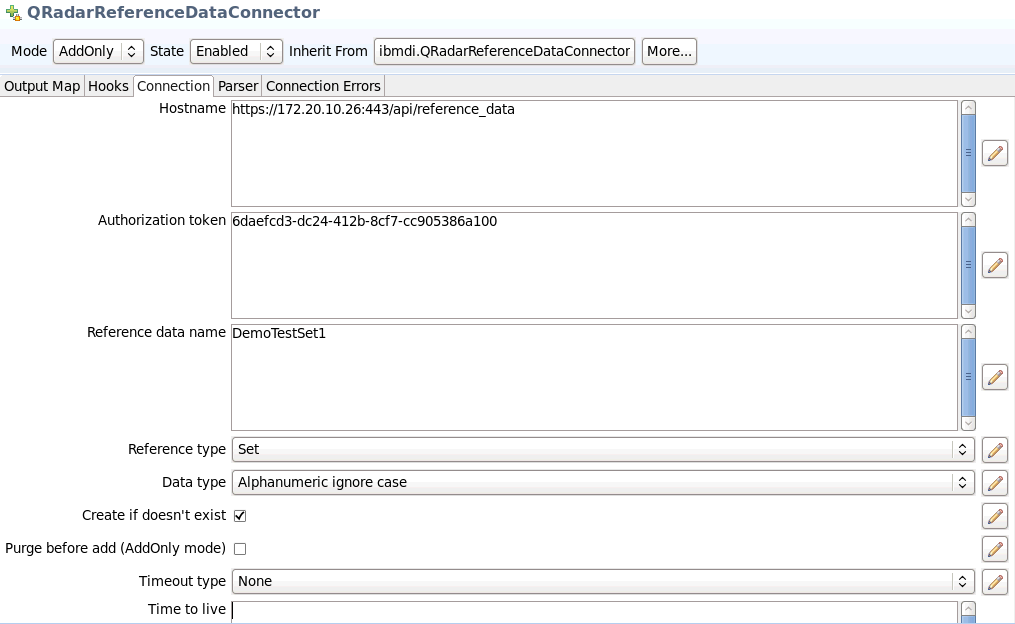
\includegraphics[width=1.0\linewidth]{figures/conn_test/parameters}
	\caption{Minta a QRadar Reference Data Connector felparaméterezésére}
	\label{fig:parameters}
\end{figure}

\begin{itemize}
	\item Hostname (szöveges mező): URL amin keresztül elérhető a QRadar reference data API-ja 
	
	\item Authorization token (szöveges mező): Token, amit a QRadarral való kapcsolódáskor az autentikációra használunk.
	
	\item Reference data name (szöveges mező): A reference data neve, amire az adatok feltöltésre kerülnek.
	
	\item Reference type (legördülő lista): A használni kívánt reference data típusa. Lehetséges értékei: Set, Map, MOS, MOM.
	
	\item Data type (legördülő lista): A reference data-ban tárolandó adatok típusa. Lehetséges értékei: Alphanumeric, Alphanumeric ignore case, Numeric, Date, IP, Port
	
	\item Create if doesn't exist (check-box): Igaz/hamis érték, azt befolyásolja, hogy a connector létrehozza-e a reference data-t, ha az még nem létezik.
	
	\item Purge before add (Add only): Feltöltés előtt törölje-e a reference data tartalmát. Ez az opció csak AddOnly mód esetén jut érvénye.
	
	\item Timeout type (legördülő lista): A Time to live paraméterben megadott értéket milyen módon értelmezze. Lehetséges értékei: None, UNKNOWN, LAST\_SEEN, FIRST\_SEEN. Azt befolyásolják, hogy honnantól számítson a time to live értéke.
	
	\item Time to live (szöveges mező): Mennyi ideig legyen elérhető az adat, a timeout type alapján. Az időtartam szöveges formátumban várja az értéket. (pl \textit{"36 hours"})
	
	\item Comment: Milyen magyarázattal kerüljön feltöltésre az adat
	
	\item Detailed log (check-box): A connector futtatásakor a naplóinformációk extra információkat is tartalmazzanak e.
	
\end{itemize} 
A QRadar connector működéséhez legalább a QRadar példány elérhetőségét, a hozzá tartozó token-t, a reference data nevét, típusát, valamint az általa használt adat típusát meg kell adni.

Végeredményképp létrehoztam a felvázolt működésnek megfelelő connector-t, ami képes a paraméterezés alapján megadott QRadar példánnyal felvenni a kapcsolatot, számára adatot feltölteni, módosítani, törölni. Ez bármilyen assembly line-ban használható, későbbi projektek során is.

\subsection{Connector működésének bemutatása} \label{subsec:conntest}
A fejlesztés következő lépése az elkészített connector tesztelése volt, valamint a helyes működés ellenőrzése. Az ennek során szerzett tapasztalatokra építve készítettem el a \ref{sec:queryk}. \nameref{sec:queryk} fejezetben leírt integrációs feladatok megoldását.

\begin{figure}[t]
	\centering	
	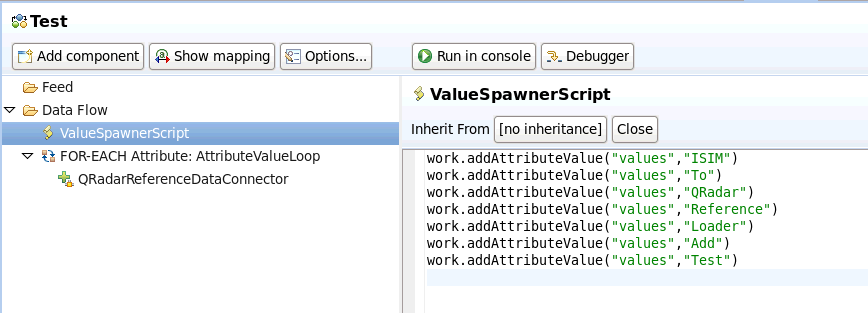
\includegraphics[width=1.0\linewidth]{figures/conn_test/connTest1}
	\caption{Adatok kézi megadása QRadar Reference data connector teszteléséhez}
	\label{fig:conntest1}
\end{figure}

A teszteléshez kézzel megadtam néhány inputot, melyeket megkíséreltem feltölteni a connector segítségével egy Reference Data-ba, majd ezeket ellenőriztem a QRadar belső menüjének használatával.
A  \ref{fig:conntest1}-es Ábrán látható, hogy egy Javascript blokk formájában feltöltöm az assembly line fő változójának értékét egyedileg definiált szövegekkel. A bal oldalon látható a teszt Assembly line, ami a feltöltő scriptből áll, a QRadar Connectorból, valamint egy ciklus vezérlőből, ami az összes string értéket egyesével továbbítja a QRadar Connector felé. 
 
 \begin{figure}
 	\centering
 	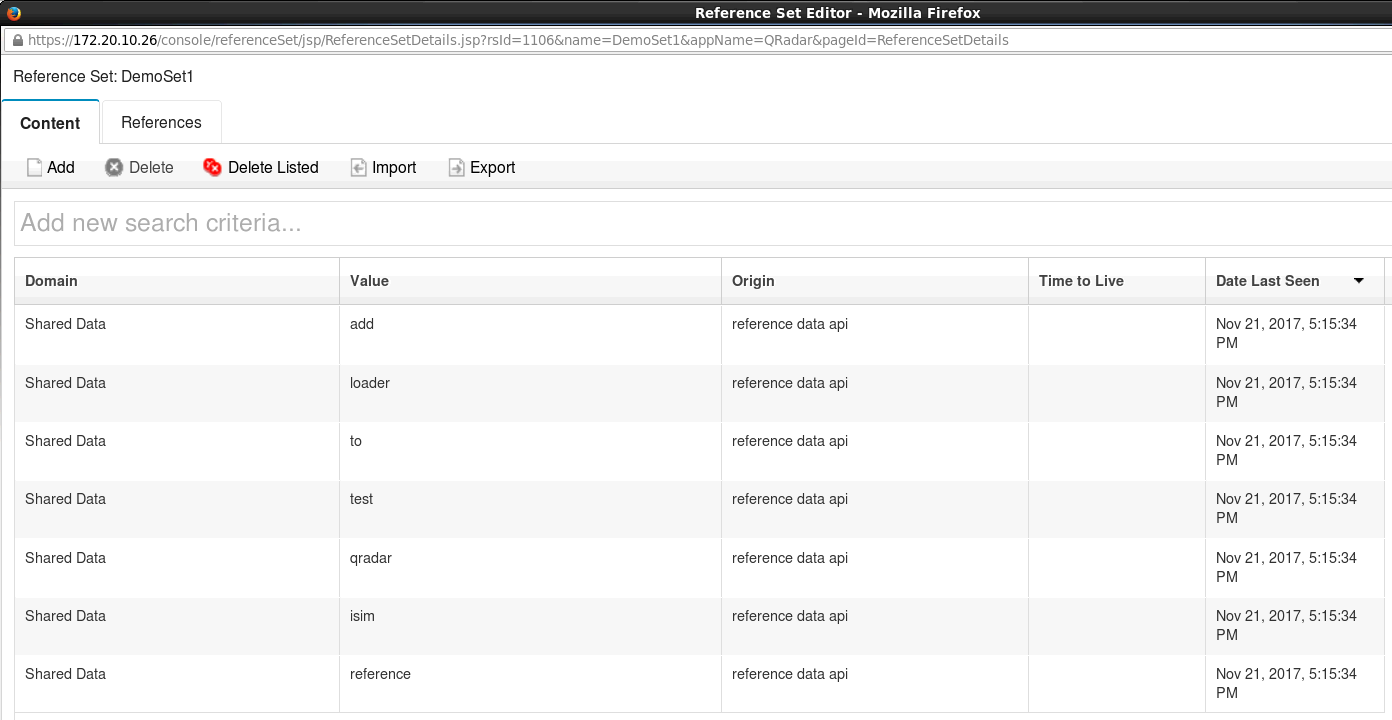
\includegraphics[width=1.0\linewidth]{figures/conn_test/qradarTest1}
 	\caption{Sikeresen feltöltött adatok a QRadar felületén}
 	\label{fig:qradartest1}
 \end{figure}
 
A folyamat eredményességét, vagyis hogy az összes általam definiált szöveg felkerült e, a QRadar reference set módosító felületén keresztül ellenőriztem. Az végeredmény a \ref{fig:qradartest1} Ábrán látható. 
 
A továbbiakban bemutatom egy példán keresztül egy integrációs feladat megvalósítását, ami az ISIM-ben található árva account-okat szinkronizálja a QRadar számára. A feladat bővebb leírása, felhasználási területei a \ref{lbl:orphanaccs} fejezetben található. 

\begin{figure}[h]
	\centering
	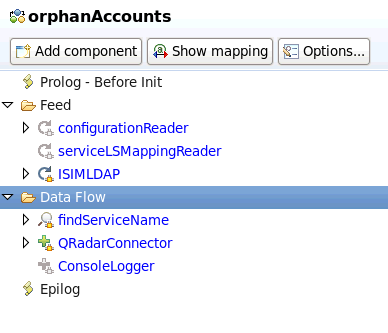
\includegraphics[width=0.6\linewidth]{figures/conn_test/queryAssemblyLineSmall}
	\caption{Személyhez nem rendelt (árva) felhasználói fiókokat összegyűjtő assembly line.}
	\label{fig:queryassemblyline}
\end{figure}

Minden TDI assembly line két főbb részből áll: a Feed-ből és a Data Flow-ból. A Feed rész tartalmazza az olyan connectorokat, amik iterator módban adatokat olvasnak fel, és ezekből új entry-ket készítenek az assembly line részére. Ezeken az entry-ken hajtódnak végre a Data Flow részben definiált connector-ok és scriptek által meghatározott műveletek.

Jelen esetben a fő adatokat az ISIMLDAP connector szolgáltatja. Ez kapcsolódik az ISIM által használt LDAP szerverhez, és felolvassa az árva accountokhoz tartozó információkat. A feedben található másik két connector kiegészítő információk felolvasására szolgál. Ezek passzív módban vannak jelen, az Assembly Line prolog scriptje ezeket felhasználva olvas be plusz információkat. A configurationReader egy property fájlból olvas be konfigurációs adatokat, a serviceLSMappingReader pedig egy másik konfigurációs fájlból olvassa fel a service DN -- QRadar log forrás név párosítást, amire azért van szükség, mert a QRadar a szabályokban logforrás neveket használ, ami nem feltétlenül ugyanaz. A külső konfigurációs fájlok használta azt teszi lehetővé, hogy ugyanaz az assembly line többféle konfiguárcióval is futtatható legyen, akár egyszerre, az assembly line módosítása nélkül.

Az account információkat tartalmazó entitásokat a Data Flow rész dolgozza fel. A findServiceName egy lookup connector, amire az accountokban tárolt információk miatt van szükség. Ugyanis az ISIM LDAP-ja az egyes accountokhoz a service-t, amihez tartoznak, egy erservice attribútumban tárolja, egy DN formájában.\cite{ldapdn} A connector ezekhez a DN-ekhez keresi meg a beszédes nevet, amit a serviceLSMappingReader connector által felolvasott párosítás indexelésére használok fel. Ezzel összeáll minden szükséges információ a feltöltéshez.

Az adat végleges formáját a QRadarConnector állítja össze, ekkor jönnek létre a \textbf{QRadar logforrás név - Account név } párosítások. Ezeket az adatokat tölti fel a megfelelő reference data-ban, jelen esetben, mivel kulcs - értékek halmaza formátumot vesznek fel az adatok, ezért egy reference map of setsbe. A futtatás eredménye a \ref{fig:orphanaccountresult} ábrán található
\footnote{A könnyebb megtekinthetőség kedvéért jelen esetben az accountok service-hez rendelését kihagytam, és egy reference setbe töltöttem be az adatokat. Ugyanis a QRadar a reference setek megtekintésére egy átláthatóbb felületet ad, mint a többihez, és így az eredmény könnyebben értelmezhető.}. 
A felsorolásban láthatók a felhasználói fiókok neveinek egy részhalmaza. Mivel a tesztrendszeren az ISIM felügyelete alatt egy linuxos rendszer található, amely sok technikai accounttal rendelkezik, így a listában főleg ezek láthatók.

\begin{figure}[h]
	\centering
	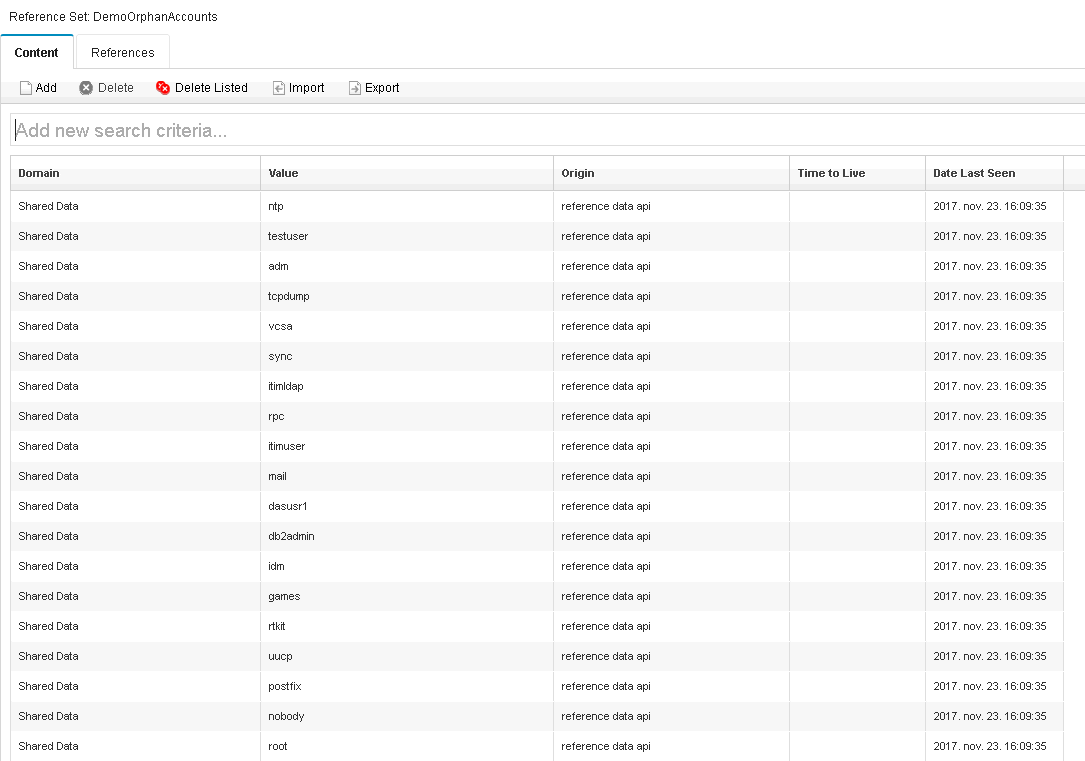
\includegraphics[width=1.0\linewidth]{figures/conn_test/orphanAccountResult}
	\caption{Árva accountok az ISIM rendszerben, melyek nagy része az egyik felügyelt Linuxos rendszerhez tartozik.}
	\label{fig:orphanaccountresult}
\end{figure}

A ConsoleLogger connector itt egy passzív állapotú connector, amit a assembly line többi eleme használ a sikeres műveletek vagy a hibák naplózására.

\section{WAS integráció megvalósítása}

Ennél a megoldásnál a cél egy robusztus alkalmazás megalkotása volt, ami jól illeszkedik egy nagyvállalati környezetbe, valamint működés és üzemeltetés szempontjából is összhangban van a hozzá kapcsolódó IBM-es termékekkel. Az előző szekcióban ismertetett TDI alapú megoldás ugyan ellátja a szükséges feladatokat, a fejlesztés egyszerű és gyors, de a használt technológiából adódik, hogy más területeken hátrányban van egy különálló, vagy akár egy menedzselt környezetben futtatott alkalmazással szemben. Ezeket a hátrányos tulajdonságokat hivatott áthidalni a WebSphere alapú megoldás.

A WebSphere alapú alkalmazás fejlesztésének főbb motivációi:
\begin{itemize}	
	\item A magas rendelkezésre állás, elosztott futtatás, egységes alkalmazásmenedzsment biztosítása.	
	
	\item Jogosultságkezelés és auditálhatóság megvalósítása. 
	
	\item Fejlesztői és üzemeltetői feladatok szétválasztása, valamint az üzemeltetési feladatok felhasználói felülettel való támogatása.
\end{itemize}

A felsorolt funkciók TDI-vel történő megvalósítása valamilyen külső megoldást kívánna, ami növelné az alkalmazás beállítási és karbantartási komplexitását, mivel ezekre is figyelmet kell fordítanunk, ezeket is ellenőriznünk kellene esetleges hibák felmerülésekor. További probléma, hogy a TDI alapú megoldás testre szabhatósága bizonyos kereteken túl nem, vagy nagyon nehezen megvalósítható. Ilyen például a felhasználói felület kérdése. A TDI alapú megoldásnál adottak az opciók: a Configuration Editor, azaz a fejlesztői alkalmazás használata, vagy a megfelelő parancssoros lehetőségek használata. Ha saját felületet akarunk készíteni, akkor nem csak annak a fejlesztését kell megvalósítanunk, de a TDI által biztosított interfészekkel való kommunikációt is. Ezzel szemben egy saját alkalmazás, menedzselt környezetben futtatva, az adott alkalmazásszerver által nyújtott lehetőségekkel együtt, a legtöbb felsorolt problémára megoldást nyújthat. 

%Az automatizált futtatást biztosítja a szerver által nyújtott ütemező, a naprakészséget és a magas rendelkezésre állóságot a szerver architektúrája és infrastruktúrája. Emellett megvalósíthatunk egyedi megoldásokat is, mint például egy egyedi logikát, ami biztosítja az elakadó szinkronizációs feladatok és az inkonzisztenciák korrigálását. A technikai és hozzáférési információkat, valamint az elosztott futtatást szintén nem kell alkalmazás szinten kezelnünk, mert a szerver tárolhatja a cache-elhető információkat és erőforrásokat, akár egy poolozott megoldással, amiket szükség esetén az alkalmazás rendelkezésére bocsájt, akár elosztottan, több példány számára is. 

A Websphere alapú alkalmazás a fenti területekre az alábbi módon kínál megoldást:
\begin{itemize}
	\item Futtatásra használhatjuk a WebSphere által kínált beépített ütemezőt, ami az általunk megadott szabályok szerint végrehajtja a feladatokat.
	
	\item Az paraméterek, valamint a feladatok elosztott végrehajtását képes a szerver kezelni, így a magas rendelkezésre állóságot elég ha a szerver szintjén biztosítjuk. Az adatok naprakészen tartásához emellett készíthetünk egyedi logikát, ami szükség esetén változtat a futtatandó feladatok során.
	
	\item Mivel az alkalmazás nem közvetlenül, hanem a szerver által biztosított kapcsolatokon keresztül csatlakozik a célrendszerhez, a költséges erőforrások poolozása könnyen támogatható, valamint biztonsági szempontból is elég a szervert biztosítani.
	
	\item Egy saját fejlesztésű, egyedi felülettel könnyen szétválaszthatók a fejlesztői, és a felhasználói feladatok a rendszer használatánál. A fejlesztő megvalósított néhány általános use case-t, amelyet a felhasználó később elér, hogy saját igényei szerint felparaméterezze, és használja őket. 
	
\end{itemize}

\subsection{Architektúra tervezése}

Mivel az alkalmazás egy projekt részeként valósult meg és többen dolgoztunk rajta, ez különösen fontossá tette az architektúra átgondolását és alapos megtervezését. 

A cél egy olyan alkalmazás fejlesztése volt, ami mind a jövőbeni fejlesztők, mind az üzemeltetéssel foglalkozó személyzet számára könnyen használható. Jelen esetben a fejlesztők alatt elsősorban azokat a személyeket értem, akik majd későbbiekben új lekérdezés (query) típusokat készítenek a rendszerhez. Ezek a személyek mélyebb ismeretekkel rendelkeznek a rendszerrel kapcsolatban, ám fontos, hogy számukra is egy könnyen használható interfészt biztosítsunk. Emellett fontos, hogy az új lekérdezés típusok könnyen, az alkalmazás minimális -- vagy optimális esetben semmilyen -- módosításával bevezethetők legyenek. Ezzel jól szétválasztható a fejlesztők és az üzemeltetők számára szükséges tudás, mivel egy már kész, új típust egy, a rendszer belső működéséhez kevésbé értő ember is gyorsan be tud vezetni. Üzemeltetői részről egy könnyen használható felület biztosítása volt a cél, ami egyértelmű tudósítást ad a rendszer állapotáról, és megkönnyíti új lekérdezések konfigurálását, azok helyes felparaméterezését.

A könnyű használat mellett fontos szempont volt, hogy az alkalmazás megfelelően robusztus legyen egy vállalati környezet számára is. Fontos cél volt az adatok naprakészen tartása mellett az adatok konziszteciájának megőrzése, valamint a megfelelő performancia elérése, de a túlterhelés elkerülése. Ezen szempontok egy része egymással ellentétes követelményekkel rendelkezik az alkalmazás számára\footnote{Például: az adatok naprakészen tartása indokolná a lekérdezések folyamatosan ismétlődő futtatását, várakozási idő nélkül, a konzisztencia pedig mindig az összes adat feltöltését. Ez azonban lassan lefutó lekérdezések esetén erősen túlterhelné a rendszert, és bizonyos, fontosabb és gyorsabb lekérdezések nem tudnának érvényesülni. A REST API túlterhelése is egy probléma, ami a feleslegesen nagy mennyiségű adat folyamatos feltöltése miatt jelentkezhet.}, így a tervezésnél kompromisszumokat kellett kötnünk.

A tervezésnél az alábbi döntéseket hoztuk:

\begin{itemize}
	\item Egységes, moduláris lekérdezésrendszer használata
	\begin{itemize}
		\item A különböző lekérdezés típusok egy közös interfészt implementálnak, ami miatt a típusok köre könnyen bővíthető utólag is.
		\item Minden ténylegesen lefutó lekérdezés egy lekérdezés típusból, és annak a felparaméterezéséből áll. Ezeket egy táblában szerializálva tároljuk, ahonnan az ütemező felolvassa, és futtatja őket.
		\item Az egyes lekérdezések felparaméterezése egy webes felületen végezhető, ami támogatja az rendszer alapján a rendelkezésre álló paraméter értékeket.
	\end{itemize}
	
	\item Két ütemező, külön időzítéssel, egy az ISIM lekérésekhez, egy a QRadar szinkronizációhoz.
		\begin{itemize}
		\item Mindkét ütemező periódusideje külön állítható, valamint a két ütemező használata miatt az összes lekérdezésnél külön állítható az ISIM lekérdezés, és a QRadar feltöltés között eltelt intervallum nagysága.
	\end{itemize}
	
	\item Kétfázisú lekérdezések, több lehetséges állapottal (Lsd.: \ref{fig:refloaderstates} Ábra)
	\begin{itemize}
		\item Minden lekérdezés két fázisból áll: egy ISIM irányú lekérési fázisból, és egy feltöltési fázisból a QRadar felé
		\item A lekérdezés létrejöttekor egy kezdeti állapotban van, majd ha az ISIM lekérdezésekhez tartozó IDM ütemező elindítja, átkerül IDM\_SYNC\_RUNNING állapotba.
		\item Ha az IDM lekérdezés sikeres volt, IDM\_SYNC\_COMPLETED állapotba kerül, ha nem, akkor IDM\_FAILED-be.
		\item Az IDM\_SYNC\_COMPLETED állapot után a lekérdezés vár, amíg az ütemező el nem indítja a QRadar irányú szinkronizációt, vagy újra sorra nem kerül az ISIM ütemező számára.
		\item A QRadar szinkronizáció futása ha sikeres, akkor COMPLETED állapotba kerül a lekérdezés. Ezt az állapotot nevezzük a sikeres végállapotnak.
		\item Ha a QRadar szinkronizáció nem volt sikeres, akkor QRADAR\_SYNC\_FAILED állapotba kerül. Ekkor a lekérdezés vár, hogy a két ütemező közül valamelyik elindítsa az egyik feladatát.
	\end{itemize}

	\item Lekérdezések eredményeinek tárolása, delta számolás
	\begin{itemize}
		\item Egy lekérdezés futtatása közben, minden sikeresen lefuttatott fázis után szerializáljuk az eredményt egy SQL adatbázisba. Emiatt ha az alkalmazás hibára futna, vagy újraindulna két fázis között, a lekérdezés eredménye megmarad.
		\item A QRadar-ra legutóbb feltöltött állapotról tárolunk egy lokális verziót, amit összehasonlítunk az ISIM lekérdezés eredményével. Ha változás történt, akkor csak a két állapot különbségét töltjük fel.
		\item Ha a különbség feltöltése közben hibára futunk, feltételezhetjük hogy a rendszeren kívülről valaki módosítást hajtott végre, és a lokális változat már nincs szinkronban. Ekkor egy teljes feltöltést végzünk az adatokkal.
	\end{itemize}

	\item Egyedi felhasználói felület fejlesztése
	\begin{itemize}
		\item Olyan felület, amelyen egyszerűen láthatók a rendszerben megtalálható, már felkonfigurált lekérdezések, valamit könnyen és gyorsan új lekérdezéseket konfigurálhatunk fel.
		\item Lekérdezések létrehozásának könnyítése sémafelderítéssel, aminek a segítségével a rendszerben található service-ek, organizációs egységek, szerepkörök, stb... listákból kiválaszthatók.
	\end{itemize}
\end{itemize}

\begin{figure}
	\centering
	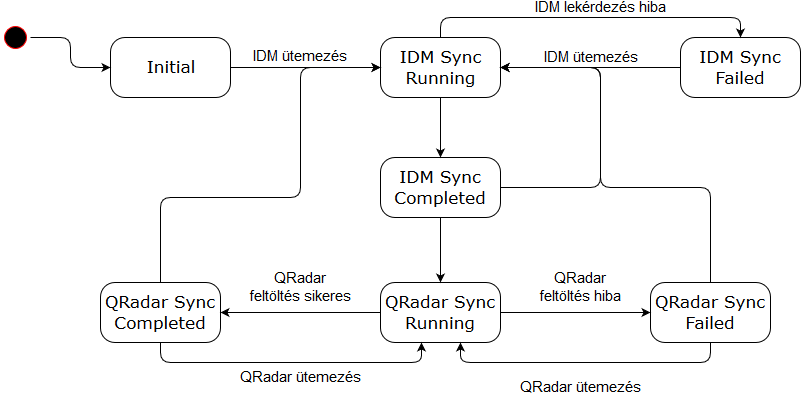
\includegraphics[width=0.9\linewidth]{figures/refloader_states}
	\caption{Egy lekérdezés futásának állapotai}
	\label{fig:refloaderstates}
\end{figure}


\section{Query-k implementációja} \label{sec:queryk}

A koncepció, valamint a fejlesztett megoldások tesztelésére az alábbi use case-eket definiáltuk:

\subsection{Felhasználói fiókok egy adott menedzselt rendszeren}
	A query célja az ISIM által kezelt egyes service-eken található összes felhasználói fiók összegyűjtése, és egy map of sets típusú reference data formájában feltöltése. 
	\subsubsection{Felhasználása} 
		Bizonyos biztonsági események tartalmazhatnak információkat nem csak arról, hogy milyen műveletet hajtottak végre, hanem azt is, hogy ki hajtotta ezt végre. Ennek azonosítása általában az adott rendszeren található felhasználói névvel történik. Ennek a query-nek az eredményeként felkerült adatok használatával ellenőrizhető, hogy az eseményben jelzett fiók az ISIM által kezelt-e. Ha nem, az annak jele lehet, hogy a fiókot a biztonsági házirend megkerülésével hozták létre, ami okot adhat biztonsági riasztásra.
		 
	\subsubsection{Megvalósítás}
		Szűrés az LDAP-ban található felhasználói fiókokra, aszerint, hogy a kiválasztott service-hez tartoznak-e.
		
		%Az ISIM az összes felhasználói fiókot egy adott LDAP részfán tárolja, eraccountitem típusú opjektumok formájában. A szervíz azonosítójára (DN-jére) az erservice nevű attribútum hivatkozik. 
		A keresést egy filterrel valósítottam meg, amelynek a kiindulási pontja a felhasználókhoz tartozó fiókokat, valamint az árva fiókokat tartalmazó részfa. Szűrési paraméternek beállítottam az alábbi filter-t: 
\begin{lstlisting}
(&(erservice=" + serviceDN + ")(objectclass=eraccountitem))
\end{lstlisting}
	Ezzel kiszűrtem az összes felhasználói fiókot (account) a rendszerben, mivel az ISIM mindegyik accountra hozzáadja objectclass-nak az eraccountitem-et. Majd ezen kívül szűrök még az erservice attribútumra, ami minden accountnál azt tárolja, hogy melyik service-en található az adott account.
	
	
\subsection{Inaktív felhasználókhoz tartozó fiókok}
	A query célja azoknak a felhasználói fiókoknak az összegyűjtése, amiknek a tulajdonosa inaktív állapotban van, és egy set formájában feltölteni. Ezek olyan felhasználók, akiket az ISIM rendszerben felfüggesztettek.
	\subsubsection{Felhasználása}
	
		Egy felhasználó felfüggesztése általában valami jogvesztéssel járó procedúra során következik be, vagy ideiglenesen, amíg nem biztos például egy jogi eljárás végkimenetele, de az időtartamára szeretnénk a felhasználót kivonni a rendszer által biztosított jogkörökből, vagy véglegesen, ha például elmegy a cégtől, és már nincs szükség az adott személy rekord-ra, valamint accountokra a menedzselt rendszereken.
		Ha azonban valamiért nem volt sikeres a kivonás, a felhasználói fiók felfüggesztése, vagy egy régebben felfüggesztett accountot újra aktiválnak valahogy, akkor egy inaktív emberhez egy aktív account tartozik, ami súlyos biztonsági rés lehet egy rendszerben.

		Ennek detektálására a SIEM biztonsági riasztást adhat, ha olyan tevékenység történik, ami a kigyűjtött, inaktív felhasználók fiókjaihoz kapcsolódik. Emellett ezek az adatok felhasználhatóak visszamenőleg is, például egy felelősségre vonási eljárásnál, egy adott személy historikus tevékenységének ellenőrzésére.
		 
	\subsubsection{Megvalósítás}
		
		Egy felhasználó aktív/inaktív státuszát az \textit{erpersonstatus} attribútum tárolja, 0 értékként ha aktív, és 1-ként ha inaktív. A felhasználókat ezen attribútum alapján szűröm, majd az eredményként kapott objektumok DN-jével létrehozok egy második filtert, ami az összes DN-t vagy kapcsolatban tartalmazza. Ennek segítségével szűrök az accountokat tartalmazó organizációs egységen.
		
		A első felhasznált filter a következő:
		\begin{lstlisting}
(erpersonstatus=1)\end{lstlisting}
		
		majd ennek az eredményét felhasználva az alábbi mintára készítek egy másik filtert:
		\begin{lstlisting}
(&(objectclass=eraccountitem)(|(owner=$PERSON_DN1$)(owner=$PERSON_DN2$)...))\end{lstlisting} \label{code:accownerfilter}
		ahol a \$PERSON\_DN\$-el jelöltem a ténylegesen behelyettesítendő, az előző filterből kapott személyekhez tartozó DN-eket.
		
\subsection{Felfüggesztési eljárás alatt álló felhasználók fiókjai}
Az előző query-nél tárgyalthoz nagyon hasonló eset, de míg az előzőnél a már felfüggesztett, tehát a befejeződött folyamatú emberekre szűrünk, itt azokra, akiknél még zajlik az eljárás. Ez általában elég ritka, mivel a felfüggesztésnek pont az a lényege, hogy gyors, atomi művelet, ami jogvesztéssel jár, de megeshet, hogy például kommunikációs, vagy adapter hiba miatt, vagy akár egy jóváhagyás miatt egy felfüggesztési eljárás nem fejeződik be.\footnote{Például egy másik, hasonlóan magas posztban álló manager emberét akarná felfüggeszteni, mert szabálysértésen kapta, de mivel azonos szervezeti szinten állnak, szükség van a jóváhagyásra a másik managertől, aki épp szabadságon van. Ekkor amíg vissza nem érkezik, addig áll a folyamat.}
	\subsubsection{Felhasználása}
		Az előző esethez hasonlóan itt is jogvesztés elmaradása áll fent, ami biztonsági réssel fenyeget. A SIEM riasztást adhat ezen felhasználói fiókok detektálásakor. 
	\subsubsection{Megvalósítás}
		Az egyik szűrő feltétel a folyamat állapota, ami a PROCESS táblában található a STATE oszlopban. A szűréshez használt értékek az 'R', 'I', 'S', amik sorrendben a Running, azaz futó, Interrupted, azaz megszakított, és Suspended, azaz felfüggesztett. A másik szűrő feltétel a process típusa, ami meghatározza hogy egy adott process ténylegesen mit hajt végre. Ez a PROCESS táblában a TYPE oszlopban található, és jelen esetben azok a folyamatok a fontosak, amik 'US' típusúak, azaz user suspend típusúak.
		
		Ezek alapján az alábbi két lépcsős folyamatban keresek először az alábbi utasítással:
		
		\begin{lstlisting}
Select REQUESTEE from PROCESS where type = 'US' and state in ('R','I','S')
\end{lstlisting}
		Ez kiválasztja a folyamat célpontját (annak is a DN-jét), az összes olyan folyamatra, ami futó, felfüggesztett, vagy megszakított állapotban van, és a típusa a már említett 'US'.
		
		Ezt követően az előző query második lekérésével megegyező formában konkatenációval készítek egy LDAP filtert, ami megadja személyekhez tartozó accountokat.
		
\subsection{Törlési folyamat alatt álló felhasználói fiókok} 
Szintén az előző query-hez hasonló eset, csak itt a törlés alatt álló accountokat keressük. Feltöltés előtt egy transzformációt hajtok végre, amivel az account halmazokat egy QRadar logforráshoz rendelem, ezzel készítve egy map of sets-t.  
	\subsubsection{Felhasználása}
		Ha egy felhasználói fiók törlése nem történik meg azonnal, 
		%Az előző esethez hasonlóan a törlés is egy jogfosztó művelet, ami ha nem atomi módon fut le, 
		hanem például valamilyen kommunikációs hiba miatt megakad, akkor egy ablak nyílik a felhasználó számára, hogy azokat a jogosultságokat használja, amelyek a biztonsági házirend szerint már nem jár neki. Ezeknek a detektálására készíthetünk szabályokat a QRadarban, amik figyelik az ilyen típusú potenciális támadásokat, és jeleznek.
		 
	\subsubsection{Megvalósítás}
		A törlési folyamattal kapcsolatos szükséges információkat a PROCESS tábla tárolja. A szükséges folyamatok összegyűjtéséhez először lekérem a  táblából azokat a rekordokat, amiknek a STATE értéke 'R','I', vagy 'S', és a TYPE értéke 'AD', azaz account delete. Ezeknek a rekordoknak a SUBJECT mezőjében megtalálható az érintett account neve, valamint a SUBJECT\_SERVICE mezőben pedig annak a service-nek a neve, amelyikhez tartozik.
		
		Utolsó lépésként egy külső fájlból betöltött QRadar logforrás - Service name hozzárendeléssel a felolvasott SUBJECT\_SERVICE alapján végrehajtom a mappelést, és így előállnak a szükséges map of set-ek.
	
\subsection{Árva fiókok } \label{lbl:orphanaccs}
Az árva fiókok olyan fiókok, melyek nem köthetők valós, a rendszerben kezelt személyhez. Ilyenek lehetnek például a rendszer által menedzselt technikai fiókok, vagy olyanok, amik korábban valós felhasználókhoz tartoztak, de valamiért megmaradtak a szétválás után is, vagy olyanok, amiket nem az ISIM-en keresztül, hanem annak megkerülésével vettek fel a menedzselt rendszeren. 
	\subsubsection{Felhasználása}
 	Az árva fiókok jelenléte komoly biztonsági rést jelenthetnek, elsősorban ha például hozzáférnek kritikus rendszerekhez, de megmaradt a alapértelmezett jelszavuk, vagy nem alkalmazták rájuk a megfelelő jelszó házirendeket, ezért fontos lehet, hogy tudjuk detektálni ezeknek a fiókoknak az összes tevékenységét, mert bármelyik fenyegetést jelenthet.
	\subsubsection{Megvalósítás}
	Az ISIM az LDAP adatbázisában ezeket a fiókokat egy külön LDAP részfában tárolja, így elég azt lekérnem. Ezt egy LDAP filterrel végzem, az így kinyert accountokat egy előre definiált map alapján hozzárendelem a megfelelő service-hez, és annak a QRadar szerinti log forrás azonosítójához.
	
\subsection{Megadott csoportokba tartozó felhasználói fiókok, menedzselt rendszer szerint}		
A query célja az összes felhasználói fiók összegyűjtése egy menedzselt rendszerről, és az adott rendszeren való csoporttagságuk alapján egy map of setsbe rendezése. A query megvalósításánál külön kihívást jelentett, hogy az egyes accountok más attribútum névvel tárolják a csoportot jelző attribútumot, így azt is külön ki kellett keresni.
	\subsubsection{Felhasználása}
		A legtöbb informatikai rendszeren létezik valamilyen felhasználói fiók csoportosítás, ami bizonyos jogköröket definiál a beléjük tartozó fiókokra,s a csoporttagságok alapján összeáll, hogy egy fiók milyen jogokkal rendelkezik az adott rendszeren. 
		
		Az egyes jogkörök általában különböző mértékben jelentenek veszélyt, ha nem megfelelő kezekbe kerülnek, így ha megvannak az adott csoportba tartozó fiókok nevei, akkor könnyen létrehozhatunk szabályokat, amiket a súlyosság szerint testreszabhatunk az alapján, hogy milyen jogokkal bírnak a fiókok, és ez milyen mértékben jelent veszélyt.
		 
		Ilyen szabály lehet például ha a privilegizált felhasználók munkaidőn kívül lépnek be, ami jelentheti akár a fiókjuk kompromittálódását is, ami széles jogkörökkel lényegesen nagyobb veszélyt jelenthet, mintha például egy végfelhasználó fiókja sérülne.
		
	\subsubsection{Megvalósítás}

		Az ISIM az alábbi architektúrát használja a service-ek és az accountok kezelésére: minden service rendelkezik egy service profile-al, ami leírja, hogy egy service típus milyen attribútumokkal rendelkezik, plusz egyéb technikai információkat tárol. Ez egy attribútum formájában adja meg, hogy a rajta található accountok milyen típusúak, azaz milyen account profile definiálja őket. Az egyes service-ekhez tartozó accountokon definiálva van egy csoportosítás, amit groupoknak nevezünk, és egy, az accounton található, többértékű attribútum értéke tartalmazza. Ennek az attribútumnak a neve azonban minden account típusra más, és ezt a nevet az egyes accountokhoz tartozó service profile-ok tartalmazzák.
		
		Ezért a megvalósításhoz egy LDAP szűréssel lekérdezem a kijelölt service-hez tartozó accountokat és az összes attribútumukat. Majd a service típusán keresztül, a service profileból lekérem a rajta található accountok csoport attribútumának nevét. Az accountokat ezután összerendelem a csoportok szerint, és elkészítem a map of setset.
	
	
\section{QRadar esemény küldő és feldolgozó fejlesztése}
A feladat motivációja, az eddig felsorolt problémákhoz hasonlóan, a QRadar monitorozási és detektálási hatékonyságának bővítése az ISIM segítségével. Az előző két implementált megoldásban az ISIM-ben tárolt felhasználói adatok egy részhalmazát tettem elérhetővé a QRadar szabályrendszere számára, mert ezek a plusz információk hasznosak lehetnek az események értelmezésében. Ezzel szemben ennél a megoldásnál az ISIM mint log forrást illesztettem a QRadarhoz. Egy ilyen megoldás már rendelkezésre állt, de az a QRadar JDBC csatlakozóját használja, ami limitált képességekkel bír (például nem join-olhatók vele táblák), és csak az ISIM-ben található audit információkat kezelte.

A fejlesztett megoldás célja más, nem audittal kapcsolatos információk küldése a QRadar számára log formájában. Ezek is fontosak lehetnek biztonsági eseményeknél, hiszen például az ISIM-ben futó/futott folyamatok információit felhasználva új incidenseket vehetünk észre. Ilyenek lehetnek jelszó változtatások (például egy széles jogkörrel rendelkező felhasználó jelszó cseréje nem várt időpontban), az ISIM szabályrendszerének változása, vagy például kézi jóváhagyás műveletek. 

A folyamatokkal kapcsolatos információkat az ISIM a saját DB2 adatbázisában tárolja. Minden folyamathoz tartozik egy rekord a PROCESS nevű táblában. Attól függően hogy az adott folyamat pontosan hogy van definiálva, lehet hogy más folyamatok is meghívódnak egy futás közben. Az egyes folyamatok konkrét implementációjával kapcsolatos információk az ACTIVITY táblában, míg a folyamat lefutásával kapcsolatos audit események a PROCESSLOG táblába kerülnek. Az események generálásakor elsősorban ezzel a három táblával dolgoztam.

A felsorolt táblákból kinyerhetők a folyamattal kapcsolatos technikai információk, mint a folyamat típusa, kezdeti ideje, általa hivatkozott egyéb folyamatok és activity-k. Emellett viszont olyan adatokat is tárolnak a táblák, amik a folyamatban résztvevő személyeket azonosítják. Ha ezeket az adatokat képes feldolgozni a QRadar oldali esemény fogadó, akkor az előzőekben ismertetett megoldás által feltöltött adatok segítségével kialakíthatók olyan szabályok, amik fontos incidenseket detektálhatnak.
 
\subsection{TDI alapú syslog küldő fejlesztése}
Az ISIM-ben található adatok feldolgozására, és ezekből syslog események generálására a már az előzőekben bemutatott TDI keretrendszert használtam. Ez kézenfekvőnek tűnt, mivel a TDI biztosít connectorokat mind az ISIM DB2 adatbázisa irányába, mind a syslog események generálásához és küldéséhez. Előbbire a Java JDBC protokollt használó JDBC connectort, utóbbira a beépített Log connectort, ami sok különböző standard logoló motor mellett a syslogot is támogatja. 

A fejlesztés első lépése a táblák és a bennük található adatok felmérése volt. Ez alapján az alábbi következtetésekre jutottam:

\begin{itemize}
	\item A PROCESS tábla az egyes folyamatok operatív információit tartalmazza. 
	
	\begin{itemize}
		\item A legfontosabb információk itt találhatók, többek közt: folyamat indítója; folyamat alanya; organizációs egység, amelyben fut; folyamat típusa és eredménye; indulási és befejezési időpont
	\end{itemize}
	
	\item Az ACTIVITY tábla sorai az egyes folyamatokhoz tartozó elemi akciók információit tartalmazza.
	
	\item A PROCESSLOG tábla a folyamat egyes lépéseinek a kiegészítő és audit információit tartalmazza.
	
	\item A három tábla közül a PROCESSLOG tábla tartalmazza az legkisebb felbontásban az folyamattal kapcsolatos információkat.
	
	\item A folyamatban résztvevő felhasználókkal kapcsolatos legfontosabb adatok a PROCESS táblában találhatók.
\end{itemize}

Ezek alapján megvalósítottam az adatok kigyűjtését a TDI segítségével. A lekérést egy 3 táblából álló join művelettel végeztem el, melyben a PROCESSLOG táblát a PROCESS táblával a PROCESS\_ID oszlopon keresztül, az ACTIVITY táblát pedig az ACTIVITY\_ID oszlopon keresztül kötöttem össze. A teljesség kedvéért mindegyik tábla mindegyik mezőjét kigyűjtöttem, további felhasználási célra. Mivel ez a TDI-ban ütközést okozott az azonos nevű mezőkön, ezért minden oszlopot a tábla nevével prefixáltam.

A következő lépés az adatok átalakítása volt a QRadar számára könnyen kezelhető formára. Mivel a feldolgozás egyik módja a reguláris kifejezések használata, így kézenfekvő volt egy olyan struktúra kialakítása, amire jól illeszthetők ilyen kifejezések. Emiatt végül az alábbiak mellett döntöttem:

\begin{itemize}
	\item Az összes attribútum összefűzése egy folytonos karakterlánccá.
	
	\item Az összes attribútum értéke elé az adott attribútum nevének hozzáfűzése. Például a PROCESSLOG tábla EVENTTYPE mezőjénél ez az alábbi formátumot eredményezte: PL\_EVENTTYPE={érték}
	
	\item Az egyes attribútumok elválasztása pontosvesszővel. Azért erre a karakterre esett a választásom, mert ezt gyakran használják ilyen célra, például az LDAP konvenciók szerint is, és pont emiatt az LDAP attribútumok értékében egy tiltott karakter, és bár közvetlenül relációs adatbázisból szelektálunk, ezek a táblák többnyire az LDAP adatbázisból kinyert, vagy ott is tárolt információkat tartalmaznak.
	
	\item Az új sor karakterek eltávolítása, valamint a nem megengedett karakterek (például pontosvesszők) backslash-el történő prefixálása az attribútumok értékeiben.
\end{itemize} 

%Ebből tehát ehhez hasonló sorok adódtak:

%RÖVIDTÁBLANÉV\_OSZLOPNÉV=ÉRTÉK;RÖVIDTÁBLANÉV\_OSZLOPNÉV=ÉRTÉK;RÖVIDTÁBLANÉV\_OSZLOPNÉV=ÉRTÉK;...


A generálási folyamat utolsó lépése a sorok felküldése syslog protokollon keresztül a QRadar megfelelő fogadó interfészére. Ehhez a beépített Log connectort használtam, egy egyedileg konfigurált Log4J logger segítségével. Az egyedi konfiguráció definiálja, hogy a beépített syslog logger legyen a használt logolási mód, milyen IP-re és portra küldjük az üzeneteket, valamint milyen formátumot használjon a logger az üzenet előállításához.

A Log4J által biztosított syslog logger azonban implementációjából fakadóan nem volt megfelelő a QRadar irányába syslog üzenetek küldésére, mivel az 1019 byte-nál hosszabb üzeneteket több üzenetté tördelte. Emiatt a QRadar a töredékeket külön eseményekként kezelte. A problémára több megoldás is kínálkozott, például egy máshogyan implementált logger használata, vagy egy saját fejlesztése, de végül a dependenciák minimalizálása, és felesleges munka elkerülése végett a QRadar egy speciális működési módját használtuk, az UDP multiline syslogot.\cite{multilnesyslog} Ennél a módnál a QRadar az ehhez definiált forrásoktól olyan üzeneteket vár, amik tartalmaznak egy egyedi azonosítót. Az azonosító felismerését egy reguláris kifejezéssel végzi a QRadar, és az értéke bármilyen karakterlánc lehet. Ennek az azonosítónak a lényege, hogy ezen keresztül azonosítja a QRadar az összetartozó tördelékeket, és a több ilyen azonosítóval rendelkező üzeneteket összefűzi egy eseménnyé.

Az UDP multiline syslog mód támogatására átalakítottam a TDI assembly line-t úgy, hogy a tördelési műveletet saját magam végzem, megadott szabályok szerint. A tényleges payloadot maximum 800 karakter méretű szeletekre tördelem, figyelve az attribútum határokat jelölő pontosvesszőkre. Így, a generált syslog header-rel együtt, az üzenetek nem haladják meg a limitet, és egyben kerülnek elküldésre. 

A szükséges egyedi azonosítókat szintén TDI-ban generálom. Mivel nem kriptográfiailag biztonságos véletlenek generálásáról van szó, hanem csak egy megfelelően nagy spektrumban egyedi azonosítókról, ezért ehhez egy egyszerű, Javascript alapú pszeudo random uuid generálást használok. Ez 8 darab 0000 - ffff értékig terjedő stringből áll, ami összesen $16^{4 * 8} $ darab egyedi kombinációt ad, ami a feladat szempontjából elégséges méretű tartományt. Ezzel a lépéssel az adatok előálltak, és a QRadar számára olvasható formátumba kerültek.


\subsection{QRadar oldali esemény fogadó fejlesztése}

A QRadar oldali fogadást a már említett UDP multiline syslog segítségével biztosítottam. Ezt egy eseményforrás felkonfigurálásánál kell megadni, és annyiban különbözik az átlagos syslog protokollon érkező üzenetektől, hogy az 514-es port helyett az 517-est használja, valamint a beérkező üzeneteknek rendelkeznie kell a már tárgyalt egyedi azonosítóval. Ha az azonosító két vagy több üzenetben megegyezik, akkor azokat a QRadar összefűzi egy eseménnyé.
\begin{figure}
	\centering
	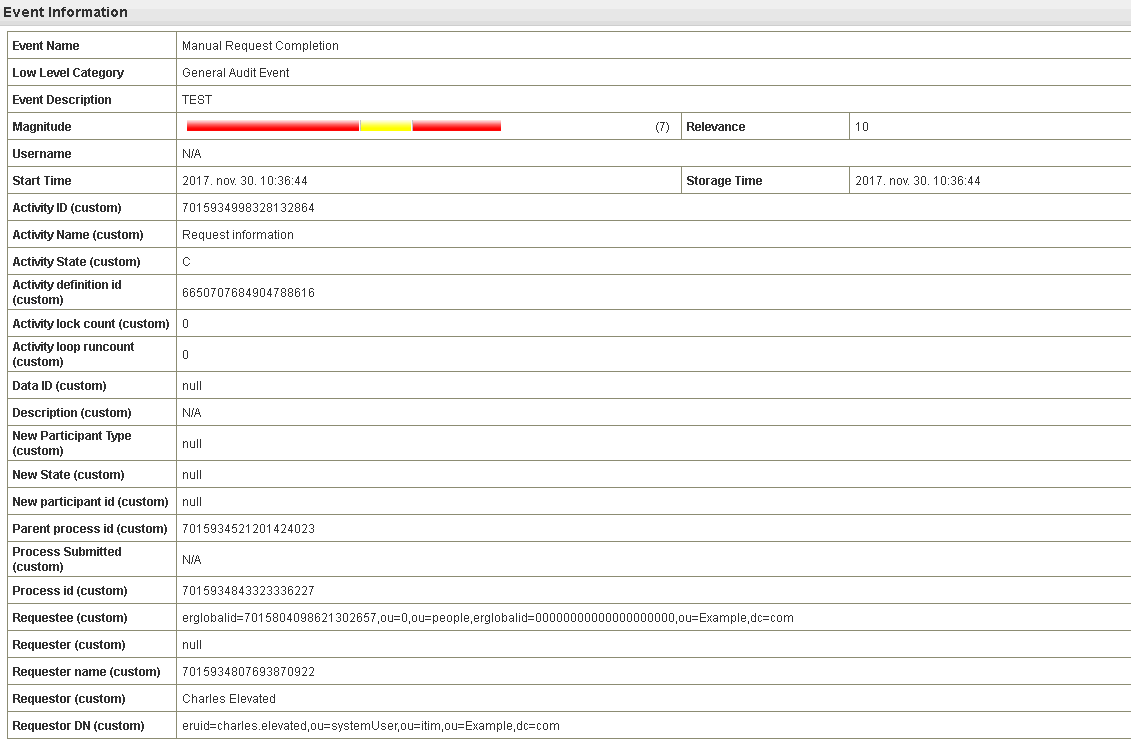
\includegraphics[width=1.0\linewidth]{figures/qradarproperties}
	\caption{Egy feldolgozott esemény a QRadar felületén}
	\label{fig:qradarproperties}
\end{figure}

Ezek alapján felkonfiguráltam egy új eseményforrást IBM Identity Manager néven, ami UDP multiline syslogokat fogad. Az egyedi azonosítók feldolgozásához egy \textit{msg\_uuid} mezőt keres a property feldolgozó, az alábbi reguláris kifejezés segítségével: 

\begin{lstlisting}
msg_uuid=(.*?[^\\]);
\end{lstlisting}

Az összeállított üzenetek eseménnyé alakításához definiáltam egy saját esemény típust, amelyet egy egyedi syslog header alapján azonosítok. A típus határozza meg, hogy a QRadar milyen szabályok szerint, milyen attribútumokat próbál meg az azonosított eseményből feldolgozni, valamint azokat hogyan használja fel a továbbiakban. Ehhez elkészítettem az összes lehetséges felküldött attribútumhoz a megfelelő reguláris kifejezést. Mivel az adatok normalizálásánál egy egységes szisztémát követtem, ezért az összes feldolgozó reguláris kifejezés az alábbi sémára épül:

\begin{lstlisting}
	ATTRIBÚTUM_NÉV=(.*?[^\\]);
\end{lstlisting}

Ennél a reguláris kifejezésnél az attribútum értéke pontosan az első találati csoportban érhető el, amibe minden karakter beletartozik, ami az attribútum nevet követő egyenlőség jel, és az első olyan pontosvessző között található, ami előtt nem backslash áll. Ezen kifejezésekkel sikerült feldolgoznom az összes lehetséges beérkező property-t, amiből a fontosabbak listája megtekinthető a \ref{tab:properties} táblázatban, valamint az összes a függelék \ref{tab:allprops} táblázatában. Az attribútum nevek felépítése a következő: az első karakter, ami a \_ előtt áll a táblát jelöli, amelyből származik (A: ACTIVITY, P: PROCESS, PL: PROCESSLOG), a \_ utáni rész pedig az adott táblában található oszlop neve. A feldolgozott esemény a felolvasott property-kkel a QRadar felületén a \ref{fig:qradarproperties} ábrán látható.

\begin{table}[!htbp] 
	\centering
	\caption{Szemelvény egy feldolgozott esemény property-jeiből.}
	\begin{tabular}{lp{10cm}}
		Attribútum név & Attribútum funkciója \\
		\toprule
		A\_COMPLETED & Az activity befejezésének időpontja \\
		A\_DESCRIPTION & Maximum 300 karakteres, beszédes leírása az activity-nek \\
		A\_NAME & Acvitiy beszédes neve. Segíti az activity azonosítását \\
		A\_RESULT\_SUMMARY & Két karakteres leírása a végeredménynek. Ezzel a mezővel szűrhetünk az activity-k végeredményére. \\
		A\_TYPE & Az activity típusa, egy karakterként tárolva. Pl: kézi (M), alkalmazás (A), subprocess (S) \\
		P\_NAME & A process neve. \\
		P\_REQUESTEE\_NAME & Annak a neve, aki számára a process végrehajtásra kerül. \\
		P\_REQUESTER\_NAME & A process kérelmezőjének a neve. \\
		P\_RESULT\_SUMMARY & A process végeredménye, két karakterként reprezentálva. Pl: jóváhagyva (AA), elutasítva (AR), sikertelen(SF). \\
		P\_TYPE & 2 karakteres kódja a process típusának. Pl: új felhasználó (UA), jelszóváltoztatás (AP). \\
		PL\_EVENTTYPE & Az adott log esemény típus kódja. Pl: activity létrehozva (AC), activity állapot változott (AS)\\
		
		PL\_REQUESTOR & Igénylő neve felhasználókkal kapcsolatos eseményeknél \\
	\end{tabular}%
\label{tab:properties}
\end{table}%

Az új esemény típus létrehozásának utolsó lépése az összerendelés definiálása, ami megadja, hogy egy adott, feldolgozott eseményt milyen attribútumok alapján, milyen típusba sorolunk. Ehhez kettő értéket használunk, amiket a QRadar minden eseménynél megpróbál feldolgozni. A két érték az Event ID, és az Event Category. Az Event ID az elsődleges klasszifikációt biztosítja. Amennyiben a feldolgozott érték megegyezik az egyik összerendelésben megadott értékkel, az egyértelműen beazonosítja az adott esemény típusát az összerendelés szerint. Az Event Category extra metadatokkal való kategorizálást tesz lehetővé az események között, olyan információkkal kibővítve az esemény feldolgozását mint az olvasható név, leírás, súlyosság, vagy alacsony- és magas  szintű kategória.

